\documentclass[12pt]{article}
\usepackage[a4paper, margin=1in]{geometry} % Set 1-inch border
\usepackage[backend=biber, citestyle=ieee]{biblatex}
\usepackage{setspace}
\usepackage{acronym}
\usepackage{float}
\usepackage{hyperref}
\usepackage{setspace}
\usepackage{lipsum} % Dummy text
\usepackage{multirow} % Table
\usepackage{tocloft}
\usepackage{quantikz}
\usepackage{booktabs}
\usepackage{fancyhdr} % Headers and footers
\usepackage{siunitx}
\usepackage{graphicx}
\usepackage{subcaption}
\usepackage{tabularx}
\usepackage{rotating}

\hypersetup{
    colorlinks=true,
    linkcolor=black,
    filecolor=black,      
    urlcolor=blue,
    citecolor=black,
    pdftitle={Thesis},
    pdfpagemode=FullScreen,
}

\addbibresource{../references.bib}

% Dots (leaders) in table of contents
\renewcommand{\cftsecleader}{\cftdotfill{\cftdotsep}}
\renewcommand{\cftsubsecleader}{\cftdotfill{\cftdotsep}}
\renewcommand{\cftsubsubsecleader}{\cftdotfill{\cftdotsep}}
\renewcommand{\thetable}{\Roman{table}}

\begin{document}
% Includes
\def\percentmem{65}
\def\percentcompute{20}
\def\percentlogic{15}

% Front cover
\title{Vision Transformer Accelerator ASIC for In-Ear Sleep Staging}
\author{Tristan Robitaille}
\newcommand{\supervisor}{Professor Xilin Liu}
\makeatletter
\renewcommand{\maketitle}{%
    \begin{titlepage}
        \onehalfspacing
        \begin{center}
            {\Large\textbf{\@title}\par}
            \vspace{2cm}
            by\par
            {\large{\@author}\par}
            \vspace{2cm}
            {\large Supervisor: \supervisor \\April 2024}
        \end{center}

        \vfill

        \begin{flushright}
        {\Huge\textbf{B.A.Sc. Thesis}}
        \end{flushright}

        \vspace{0.1\baselineskip}

        \begin{spacing}{0.4}
        \begin{flushright}
        \rule{3.25cm}{0.3pt}\\
        \rule{3.25cm}{0.3pt}\\
        \rule{3.25cm}{0.3pt}\\
        \rule{3.25cm}{0.3pt}
        \end{flushright}
        \vspace{-2\baselineskip}
        \rule{\textwidth}{0.3pt} 
        \rule{3.25cm}{0.3pt} \hspace{\textwidth-6.75cm} \rule{3.25cm}{0.3pt}\\
        \rule{3.25cm}{0.3pt} \hspace{\textwidth-6.75cm} \rule{3.25cm}{0.3pt}\\
        \rule{3.25cm}{0.3pt} \hspace{\textwidth-6.75cm} \rule{3.25cm}{0.3pt}\\
        \rule{3.25cm}{0.3pt} \hspace{\textwidth-6.75cm} \rule{3.25cm}{0.3pt}\\
        \rule{3.25cm}{0.3pt}\\
        \rule{3.25cm}{0.3pt}\\
        \rule{3.25cm}{0.3pt}\\
        \rule{3.25cm}{0.3pt}
        \vspace{2.5\baselineskip}
        \end{spacing}
        \begin{figure}[H]
            
\includegraphics[width=10.5cm]{assets/div_engsci_logo.pdf}
        \end{figure}
    \end{titlepage}
}
\makeatother
\maketitle

% Flyleaf
\newpage
\thispagestyle{empty}
\vspace*{\fill}
\begin{center}
\Large
This page intentionally left blank.
\end{center}
\vspace*{\fill}

\onehalfspacing

% Title
\newpage
\begin{titlepage}
    \thispagestyle{empty}
    \centering
    {\LARGE\bfseries ESC499 Engineering Science Thesis\par}
    {\Large Vision Transformer Accelerator ASIC for In-Ear Sleep Staging\par}
    \vspace{8cm}
    {\Large Tristan Robitaille\par}
    {\textit{Student number}: 1006343397\par}
    {\textit{Email}: tristan.robitaille@mail.utoronto.ca\par}
    \vspace{5cm}
    {\large Supervisor: Professor Xilin Liu\par}
    {\textit{Email}: xilinliu@ece.utoronto.ca\par}
    \vspace{2cm}
    {\large April 12th, 2024\par}
    \vspace{2cm}
    \begin{center}
        \copyright\ 2024 Tristan Robitaille
    \end{center}        
\end{titlepage}
\newpage

\pagenumbering{roman}
% Abstract
\section*{Abstract}
Insomnia is a wide-spread sleep disorder affecting hundreds of million of people worldwide. New treatments are being developed to address this issue, including neuromodulation,
which aims to modify nervous activity in the brain to improve sleep quality. Effective neuromodulation requires live, practical and accurate assessment of the user's sleep stage.
The state-of-the-art for sleep staging involves polysomnography, which may require up to 24 sensors, technician supervision and manual annotation by a sleep expert for the
most accurate results. Needless to say, polysomnography is not suitable for widespread, frequent, at-home use. Wearable devices, such as in-ear sensors, may be able to provide
automatic sleep staging. In this work, we investigate the feasibility of running an AI model in-ear via an ASIC accelerator for automatic sleep staging. This thesis present a vision
transformer-based model achieving 82.9\% accuracy on the MASS SS3 dataset with a model size of 31.59kB. It also develops an ASIC accelerator to measure the power, area and latency
cost of running such a model. The accelerator consumes 3.046mW on average, has an area of 3.86$mm^2$ and an inference latency of 6.97ms. The results show that the accelerator is 
viable for in-ear use in all aspects except area. Further work is suggested to reduce the power consumption and area of the accelerator by 72.2\% and 54.8\%, respectively.
\newline
\newline
{\bf Keywords:} Sleep staging, ASIC accelerator, vision transformer, computer architecture
\newline
\newline
{\bf Note:} The code is available on my GitHub repository: \href{https://github.com/TristanRobitaille/engsci-thesis}{TristanRobitaille/engsci-thesis}
\newpage

% Acknowledgements
\section*{Acknowledgements}
I would like to express my gratitude to my supervisor, Prof. Xilin Liu, for his guidance and support throughout the project. He has given me the freedom to explore new ideas and had provided me with the
support and tools I needed.

I would also like to thank my father, Claude Robitaille, for letting me remotely use his workstation to train the model and run the accuracy study. He has also helped review the code for the functional simulation.

In addition, I owe much to the professors who have taught me the fundamentals of computer architecture at the University of Toronto - Profs. Jason Anderson, Natalie Enright-Jerger, Andreas Moshovos and Mark C. Jeffrey.

Throughout this project, I have made extensive use the Compute Canada cluster, which has provided me with the computational resources I needed to run the simulations and train the model. I would like to thank the 
staff at Compute Canada for their initiative. I am also appreciative of the tools provided by the Canadian Microelectronics Corporation, which have been instrumental in the hardware implementation of the accelerator.

I would also like to acknowledge the work of Professors Lisa Romkey and Alan Chong who organized this thesis project for us, ensuring a structured and productive environment.

Finally, I would like to thank my family and friends for their support and encouragement throughout this project. I am grateful for their patience and understanding during this time.

\newpage

% Table of Contents
\tableofcontents
\newpage

% List of Figures
\listoffigures
\newpage

% List of Tables
\listoftables
\newpage

% List of abbreviations
\section*{List of Abbreviations}
\begin{acronym} {
    \small\setstretch{0.8}
    \acro{adc}[ADC]{Analog-to-Digital Converter}
    \acro{afe}[AFE]{Analog Front-End}
    \acro{ai}[AI]{Artificial Intelligence}
    \acro{asic}[ASIC]{Application-Specific Integrated Circuit}
    \acro{bvp}[BVP]{Blood Volume Pulse}
    \acro{cim}[CiM]{Compute-in-Memory}
    \acro{cmos}[CMOS]{Complimentary Metal Oxide Semiconductor}
    \acro{csv}[CSV]{Comma-Separated Values}
    \acro{ecg}[ECG]{Electrocardiography}
    \acro{eeg}[EEG]{Electroencephalography}
    \acro{emg}[EMG]{Electromyography}
    \acro{eog}[EOG]{Electrooculography}
    \acro{fsm}[FSM]{Finite State Machine}
    \acro{gsr}[GSR]{Galvanic Skin Response}
    \acro{hdf5}[HDF5]{Hierarchical Data Format 5}
    \acro{ip}[IP]{Intellectual Property}
    \acro{isa}[ISA]{Instruction Set Architecture}
    \acro{mac}[MAC]{Multiply-Accumulate}
    \acro{mass}[MASS]{Montreal Archive of Sleep Studies}
    \acro{mhsa}[MHSA]{Multi-Head Self-Attention}
    \acro{mlp}[MLP]{Multi-Layer Perceptron}
    \acro{nmos}[nMOS]{N-Channel Metal Oxide Semiconductor}
    \acro{pe}[PE]{Processing Element}
    \acro{ppa}[PPA]{Power, Performance and Area}
    \acro{psg}[PSG]{polysomnography}
    \acro{rtl}[RTL]{Register Transfer Level}
    \acro{stages}[STAGES]{Stanford Technology Analytics and Genomics in Sleep}
    \acro{tpu}[TPU]{Tensor Processing Unit}
    \acro{tsmc}[TSMC]{Taiwan Semiconductor Manufacturing Company}
    \acro{vcd}[VCD]{Value Change Dump}
    \acro{rnn}[RNN]{Recurrent Neural Network}
    \acro{cnn}[CNN]{Convolutional Neural Network}
    \acro{dnn}[DNN]{Deep Neural Network}
}
\end{acronym}
\newpage

% Body
\pagenumbering{arabic}

\section{Introduction}
\label{sec:intro}
As reported by Chaput \textit{et al.} \cite{insomnia_prevalence}, insomnia impacts around 24\% of Canadians adults. Detection and classification of sleep stages, known as
\textit{sleep staging}, followed by neuromodulation has been recently found by Yoon \cite{yoon2021neuromodulation} to be a promising treatment against insomnia. The current
stage-of-the-art for sleep staging involves the use of polysomnography to measure biosignals (at least 19 sensors are required, as explained by Levin and Chauvel \cite{RUNDO2019381})
and manual annotation by a sleep expert, which requires, on average, 2 hours of work \cite{phan2022automatic}. This technique also does not provide neuromodulation. To address
these downsides while effectively treating insomnia, we propose an in-ear device performing \ac{eeg} sensing, sleep staging and neuromodulation. To maximize treatment potential,
the device should be as small and portable as possible such that it can be used at home.

This thesis focuses on the development of a deep learning model to perform sleep staging and on the design of an accelerator ASIC module to perform in-situ inference with said
model. In the end, it aims to prove, by simulations, the viability of such an accelerator in order to potentially integrate it in the in-ear device. Multiple authors
\cite{dutt2023sleepxai, fu2021deep, eldele2021attention} have published high-accuracy results using a deep learning approach to sleep staging, and have done so with significantly
fewer sensors than polysomnography. However, these AI models run on standard computers as software frameworks and are thus unsuitable for a lightweight, integrated solution.
Google sells small custom AI-accelerators (such as the Coral Edge TPU) that could run these AI models, but they still consume too much power (at least 1W, \cite{coral_datasheet})
and do not readily integrate with custom neuromodulation hardware.

The proposed solution should match the accuracy of traditional polysomnography and published models in the literature with a power consumption low enough that the whole system
can be powered for at least a full-night on a battery that fits in-ear. The silicon area of the accelerator should allow it to fit, along with the rest of the system, on an integrated
circuit fit for integration in an earbud-type device. This document provides an overview of the literature in both automatic sleep staging using \ac{ai} and in \ac{asic} accelerator
design, establishes technical requirements for the device, describes the model used and hardware design, evaluates their performance and discusses improvements and future work.
\newpage

\section{Problem Statement and Technical Requirements}
\label{sec:prob_statement}
In light of the background of Section \ref{sec:intro}, the problem statement of this thesis is to develop a deep learning model and an ASIC accelerator for automatic sleep staging
in order to determine whether such a system can be used in an earpiece-type device for automatic sleep staging. The results of this thesis will guide future development in the field.

Table \ref{tab:design_goals} indicates precise design goals and their justification, which helps guide design decisions and development effort. For example, to reach the target
model size, time will be spent evaluating the impact of hyperparameters to find the combination that gives the lowest size while meeting the desired accuracy. For the AI accelerator,
since inference power and clock frequency are inversely proportional, we must focus on reducing energy per inference. From first principles, this implies reducing the amount of
charge that is displaced within the chip. Since the physical properties are locked for the target 65nm node, we focus on reducing the number of operations, simplifying operations,
limiting data movement and reducing control logic.

To determine the average power consumption constraint, the battery capacity of the Airpods Pro, which was found in a teardown to be 0.16Wh, can be considered as a reference
\cite*{AirpodsIfixitTeardown}. Assuming a goal of 10h of battery life (for a full night of sleep), the overall power consumption must stay below 16mW, on average. The speaker coil
driving circuitry will consume most of the power and, leaving enough power budget for the analog front-end and overhead in the system, in addition to a safety factor, 5mW seems
like a reasonable target for the accelerator. Regarding the target area and model size, a reasonable chip package for this application is a 4mm x 4mm Chip-Scale Package (CSP).
According to IPC standard J-STD-012, a CSP overall area is no more than 120\% of the die, which leaves 13$mm^2$ of die area \cite*{J_STD_012}. To further contextualize, Apple's
H1 processor, which is used in the Airpods Pro, has a similar die area of 12$mm^2$ \cite*{H1DieSize}.

Again, a significant portion will be consumed by the coil driver, RISC-V processor and memory. Therefore, a maximum area of 15\%, or 2$mm^2$, for the accelerator seems to be a safe
option. According to Liu and Kursun, the area of a standard 6T SRAM cell is 0.75$\mu m^2$ \cite*{liu2008characterization}. To leave enough area for the compute elements, controllers
and routing, reserving 0.75$mm^2$ of the accelerator area to weights is reasonable. This provides up to 1Mb, or 125kB, ignoring memory access overhead, for the weights of the model.
Finally, as mentioned above the accuracy should be close to published literature in this field to provide effective treatment. For this, 80\% is a reasonable goal. Current \ac{psg}
divides the night in 30s ``sleep epochs''. To limit too much of an offset between the end of a 30s epoch and its predicted sleep stage (essentially a phase offset), which would add
inaccuracy to the overall system and potentially reduce its effectiveness, a maximum phase offset of 10\% (3s) is appropriate. Finally, a clock of 200MHz is a typical upper-bound
for low-power microcontroller-type systems. To avoid needing two separate clock domains, which entails more area and power, the accelerator should be able to run at 200MHz.

\begin{table}
    \centering
    \renewcommand{\arraystretch}{1.2} % Vertical spacing
    \setlength{\arrayrulewidth}{1.5pt} % Thickness of vertical lines
    \caption{Design goals for AI model and ASIC accelerator}
    \begin{tabular}{@{} *7l @{}}
        \toprule
        Type        & Goals                                     & Justification &&&  \\\midrule
        \multirow{2}{*}{Model}
                    & Size $<$ 125\,kB                          & Help reach ASIC area/power goals \\
                    & Accuracy $>$ 80\%                         & Competitive with state-of-the-art \\ \bottomrule
        %%%%%%%%%%%%%%%%%%%%%%%%
        \multirow{3}{*}{ASIC}
                    & $P_{\mathrm{avg}} < 5\,\mathrm{mW}$       & System to function for whole night \\
                    & $A_{\mathrm{total}} < 2\,\mathrm{mm}^2$   & Fit in ear (65nm node) \\
                    & $T_{\mathrm{inference}} < 3\,\mathrm{s}$  & Maximum phase offset of 10\% \\
                    & $f_{\mathrm{Max}} > 200\,\mathrm{MHz}$    & Compatibility with rest of system \\
        \hline
    \end{tabular}
    \label{tab:design_goals}
\end{table}

\newpage
\section{Literature Review}
\subsection{Machine Learning for Sleep Staging}
Deep learning for sleep staging has been studied since around 2017. Broadly speaking, basic \ac{dnn} cames first, followed by \ac{cnn} and \ac{rnn} \cite{phan2022sleeptransformer}. The transformer
is a relatively new type of neural network based around the concept of ``attention'' and particularly suited for sequence inputs since it can process the input in parallel \cite{han2022survey}.
Since its introduction in 2017 \cite{vaswani2017attention}, the transformer has been used for sleep staging tasks. Indeed, Dai \textit{et al.} developed a transformer-like model without decoders
which used three input EEG channels and achieved 87.2\% accuracy on the popular SleepEDF-20 dataset \cite{dai2023multichannelsleepnet}. Similarly, Phan \textit{et al.} developed a model with a
focus on outputting easily-interpretable confidence metrics for clinicians. They found that a significant impediment to the adoptation of automatic sleep staging in clinics is lack of trust from
clinicians as they perceive the system to be a ``black box''. Their model ingests multiple sleep epochs for each inference, which allowed the team to achieve 84.9\% accuracy on the SleepEDF-78
dataset. Eldele \textit{et al.} managed an accuracy of 85.6\% on SleepEDF-78 using a single-channel, single-epoch attention-based model \cite{eldele2021attention}.

In recent years, the accuracy of sleep staging by ML models has plateaued. In fact, Phan \textit{et al.} claim that AI-based sleep-staging in heathly patients has been solved fully as the
accuracy has reached the ``almost perfect'' level of Cohen's kappa \cite{phan2022automatic}. However, none of the models presented above meet our constraints. Indeed, we require a lightweight,
single-channel, single-epoch model. Most models have more than 1M parameters \cite{phan2022sleeptransformer}; even the smallest model by Eldele \textit{et al.} has above 500k 32-bit float
weights, which far exceeds the 125kB constraint. Furthermore, none have been optimized to run on custom hardware. Thus, there is a need to develop a novel lightweight transformer.

% Lit review: AI accelerator ASIC
\subsection{AI Accelerator Hardware}
AI accelerators are a very active area of research at the moment. Significant gains in latency and power are possible by designing hardware optimized for machine learning. Indeed, CPUs
lack in memory bandwidth and parallelism and have significant control overhead as required to process any arbitrary program. GPUs have high cost and high power consumption and typically have
less available memory than a CPU. Hardware (FPGA and ASICs), on the other hand, can be fast and energy efficient but suffer from limited flexibility \cite{hu2022survey}. The first AI accelerator
ASIC, publised in 2014 by Chen \textit{et al.} and named \textit{DianNao}, could perform 452G 16b fixed-point computations per second \cite{chen2014diannao}. It was quickly surpassed by
\textit{ShiDianNao}, which was 1.87x faster and used 60x less energy \cite{du2015shidiannao}.

Modern models are massive and suffer from memory access penalties. Thus, the most optimized architectures limit data movement as much as possible by placing the compute elements directly
\textit{in memory}, meaning that less charge is switched per operation (DRAM access requires 200x more energy than on-chip memory \cite*{ding2017circnn}) and the overhead and bottleneck effect
of the data bus is drastically reduced. For example, Arora \textit{et al.} describe ``CoMeFa'', a \ac{cim} module for FPGA BRAM which managed to reduce energy comsumption by 55\%. They placed up
to 160 single-bit processing element per BRAM (20kbit) and perform operations in a bit-serial manner instead of the traditional bit-parallel \cite*{arora2022comefa}. Similarly, Wang and colleagues
presented a similar BRAM CiM module which sped up compute by up to 2.3x at the cost of 1.8\% increase in area \cite*{wang2021compute}. A high-level architecture that often uses a number of \ac{cim}
is known as ``dataflow''. Unlike the traditional von Neumann architecture, it does not rely on instructions and banks of memory cells to perform the necessary computation, but instead organizes
different compute elements sequentially and in parallel to match a model's architecture. For instance, Farabet \textit{et al.} present a runtime-reconfigurable dataflow architecture based on nine 
pipelined ``processing tiles'' that can be reconfigured in $\sim$$10^4$-$10^5$ permutations \cite{farabetlargescale}.

Another area of research is concerned with the software-hardware co-design opportunities afforded by tight integration between the model and the hardware running its inference. Ding and team
describe an impressive design where both the training backpropagation and inference hardware are modified. By ensuring that weight matrices consist of an array of circulant matrices, the team
is able to reduce time-complexity of vector-matrix mutliply from $\mathcal{O}(n^2)$ to $\mathcal{O}(n\log{}n)$. This technique reduced storage needs by 400x-4000x, enabling the model to be stored
in on-chip memory and reducing energy consumption by 60x-70x compared to naïve FPGA implementation \cite*{ding2017circnn}. Taking a different route, by developing a so-called ``Block-Balanced Pruning'' 
technique to pack a pruned weight matrix and its index information in an FPGA BRAM, Qi \textit{et al.} managed to double inference speed compared to a GPU \cite*{qi2021accommodating}. Another example
of software-hardware co-design is the work by Zhi \textit{et al.} who developed a ``Clipped staircase ReLU'' activation function optimized for their custom CiM processing element and use of quantized
weights. Their work consumed 5x less energy and 100x-1000x fewer memory accesses \cite*{zhi2021opportunities}.

\subsection{Lessons From The Literature}
The literature reviews presented above offer promising design directions to help reach the design goals. Firstly, a small model is critically missing from the literature since even the smallest
model is 16x too large for our project. Secondly, CiM and dataflow architectures are proven techniques to decrease power consumption and offer promising inspiration for the design of the ASIC.
Finally, good software-hardware co-design should not be overlooked as it can offer significant gains.

\label{sec:lit_review}

\newpage
\section{How to Design an AI Accelerator}
\label{sec:methods}
This section describes the workflow used for this project, which was divided into three main steps: model prototyping, accelerator functional simulation and accelerator hardware implementation.
The tools used in each step are described in the following sections. The goal is to expose progressively more layers of abstraction to make hardware/software co-design and debugging easier. As
can be seen in Figure \ref{fig:workflow}, these three steps allow iterations to converge on a design that meets the requirements.
\begin{figure}[H]
    \centering
    \caption{Three step workflow for designing an AI accelerator}
    \includegraphics[width=0.9\textwidth]{assets/workflow.png}
\end{figure}
\label{fig:workflow}

\subsection{Model Prototyping, Data Processing and Accuracy Measurements}
The first step in designing an accelerator is prototyping the model that the accelerator will run. Here, we prioritize productivity of development and profiling over performance. In this project,
the model was developed in TensorFlow, a widely-used Python framework maintained by Google. Its popularity implies that it has a large community of developers and is well-documented. TensorFlow
also provides a high-level API that allows for rapid prototyping of models.
The model was developed in Python 3.11 and TensorFlow 2.14. The model was trained on the \ac{mass} SS3 dataset, which contains 62 nights of \ac{psg} recordings with 21 \ac{eeg} channels \cite*{SP3/9MYUCS_2022}.
The 16-bit raw \ac{psg} data was preprocessed manually with the following steps:
\begin{itemize}
    \item Pruning of epochs of unknown sleep stage.
    \item Downsampling from 256Hz to 128Hz to reduce model size and inference energy.
    \item Filtering with 60Hz notch filter to remove noise from AC mains coupling.
    \item Filtering with 0.3-100Hz bandpass filter to remove noise (as recommended in \cite{supratak2017deepsleepnet}).
    \item Offset by half of the scale to replicate the unsigned 16-bit format expected from the \ac{adc} in the final hardware.
\end{itemize}
In addition, the two light sleep stages (N1 and N2) were merged into one stage to simplify the model. Finally, the nights were concatenated and shuffled.
All training and hyperparameter search took place on the Compute Canada Cedar cluster through remote SSH access.

Accuracy against \ac{psg} ground truth was assessed through repeated 31-fold validation: the model is trained on 60 nights and tested on the remaining two nights. The best accuracy of 5 runs is recorded, and 
the process is repeated another 30 times until all pairs of nights have been tested. The training set represents 90\% of the 60 training nights. The final accuracy is the average of the best accuracies of each
validation fold. This provides measurements that are robust against night-to-night variability in the dataset and resulting inference performance. Table \ref{tab:training_hyperparameters} shows the
hyperparameters used for training the model. These have been empirically determined to yield the best accuracy with reasonable training time. Figure \ref{fig:acc_vs_epoch} shows the accuracy of the model as a
function of the number of epochs, which is shown to converge at around 100 epochs.

\begin{table}[ht]
    \centering
    \renewcommand{\arraystretch}{1.2} % Vertical spacing
    \setlength{\arrayrulewidth}{1.5pt} % Thickness of vertical lines
    \caption{Training hyperparameters for vision transformer model}
    \begin{tabular}{@{} *5l @{}}
        Hyperparameter                  & Value &&&     \\\toprule
        Learning rate schedule          & $\sqrt{d_{model}}*min(\sqrt{step}, step/4000^{1.5})$ \\
        Initial learning rate           & 0.001        \\
        Batch size                      & 16            \\
        \# of epochs                    & 100           \\
        Dropout rate                    & 30\%          \\
        Class weights                   & 1.0 $\forall$ \{Wake, REM, N1/N2, N3/N4\} \\
        Optimizer                       & Adam          \\
        Data downsampling               & 256Hz → 128Hz \\
        Data filtering                  & 60Hz notch → 0.3-100Hz bandpass → 16b quantization \\            
        \hline
    \end{tabular}
    \label{tab:training_hyperparameters}
\end{table}

\begin{figure}
    \centering
    \caption{Testing set accuracy for 5 randomly-selected folds as a function of epoch}
    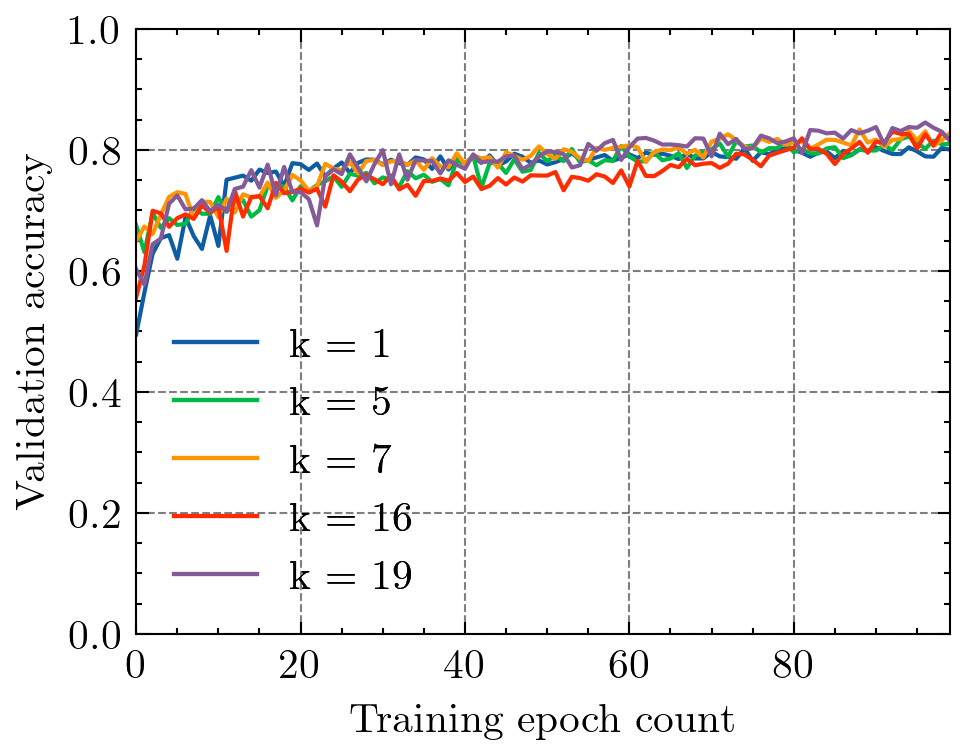
\includegraphics[width=0.9\textwidth]{assets/acc_vs_epoch/acc_vs_epoch.png}
\end{figure}
\label{fig:acc_vs_epoch}
\subsection{Accelerator Functional Simulation}
To prototype the accelerator architecture, run more accurate studies to determine the impact of design choices and write the model in a way that can be easily translated to 
hardware, a functional simulation was written. The simulation is written in C++ and, in the aim of helping subsequent SystemVerilog development, uses a similar structure to
the SystemVerilog code (cycle-level parallelism, use of FSM, limited function calls). It is organized identically to the hardware design, with a \texttt{master} module controls
high-level operation of \texttt{CiM} modules. It also makes use of compute modules written using the same fixed-point format and approximation as the hardware. This functional 
simulation is used to collect metrics that are difficult to measure in hardware, such as the distribution of inputs to certain operations, the distribution of intermediate results,
the exact number of all types of operations, etc. This information can be used to optimize the hardware design. Finally, it provides an easy way to validate the operations by
cross-checking each step with reference outputs from the TensorFlow model. The only non-standard libraries used are \texttt{armadillo} for compute verification, \texttt{HighFive}
for \ac{hdf5} file I/O (storing model parameters and \ac{eeg} data) and \texttt{rapidcsv} for \ac{csv} file I/O (storing fixed-point accuracy study results).

\subsection{Accelerator Hardware Implementation}
The final step in the workflow is the hardware implementation of the accelerator. The hardware is written in SystemVerilog and uses the same structure as the functional simulation.
Several tools are used to design the hardware:
\begin{itemize}
    \item Verilator: \ac{rtl} compiler and linter.
    \item CocoTB: Python testbenching framework.
    \item Gtkwave: \ac{vcd} waveform viewer.
    \item ARM Artisan Physical IP: SRAM compiler.
    \item Synopsys Design Compiler: Synthesis and performance evaluation tool.
\end{itemize}
The first three tools are open-source and compatible with all major operating systems, providing a familiar, local and OS-agnostic development environment. The last two tools
are proprietary and are used to evaluate the performance of the design against requirements.


\newpage
\section{Vision Transformer Model Design}
\label{sec:vision_transformer}
This section describes the architecture of the vision transformer model used in this thesis, which is shown Figure \ref{fig:vit}. Since sleep staging as presented
here is a ``sequence-to-one'' problem, feedback is not applicable and thus the decoder stack present in a more traditional transformer is not needed. The patch divide step and
first dense step (known as ``patch projection'' in \cite{dosovitskiy2010image}) are performed as data comes in from the \ac{eeg} \ac{adc} to reduce temporary storage usage. The 
patch divide step splits the input into 60 patches of 64 samples. The resulting nearly square matrix helps maximize utilization of the accelerator described in Section \ref{sec:arch},
yielding shorter inference time and lower inference energy. The patch projection step adds a layer of learned weights to the input to allow the model to capture more complex features
from the input waveform. The projection depth is known as ``embedding depth'' or \texttt{d\_model} and is a hyperparameter of the model. The model uses an embedding depth of 64,
which was determined through hyperparameter search to yield accuracies similar to embedding depths of 32 or 128 (see Figure \ref{fig:emd_depth_acc}) but offers lower energy consumption
when paired with 60 patches due to increased utilization. This is discussed further in Section \ref{sec:sw_hw_co-design}. The model then applies a learned 1D positional embedding to
the patches to allow the model to learn positional infromation of the \ac{eeg} stream. The model then applies a single encoder layer consisting of \ac{mhsa} and \ac{mlp} layers. Figure
\ref{fig:enc_layer_acc} shows that accuracy does not increase as more encoder layers are added, so the model uses only one encoder layer to reduce the model size. The LayerNorm layers
first normalize the inputs to a Gaussian over the second dimension, and then scale and shift the normalized values using learnable parameters ($\gamma$ and $\beta$, respectively) with
the goal of faciliting learning and containing compute unit inputs throuh reducing covariate shift. The \ac{mhsa} layer uses a triplet of three-dimensional weights (known as ``key'', 
``query'', ``value'') to favour certain regions of the encoder input. The \ac{mhsa} layer contains the majority of the weights in the model and is the most computationally expensive
part of the model. The third dimension of the weights is known as the ``number of heads'', and the model uses 8 as it was found to yield the highest accuracy as seen in Figure 
\ref{fig:att_heads}. The MLP head layer is a simple parametrized sequence of dense layers. Here, a single matrix was found to yield the highest accuracy. The final dense and softmax
layers are used to map the model output to the sleep stage classes. Finally, the model takes the window average of the last three softmax vectors to stabilize the sleep stage noise.
This addition has increased the model's accuracy by 2.5\% and is a novel technique in sleep staging models. Table \ref{tab:model_param} summarizes the hyperparameters of the model.

\begin{figure}
    \centering
    \caption{High-level transformer architecture for in-situ sleep staging}
    \includegraphics[width=0.65\textwidth]{assets/vit.png}
    \label{fig:vit}
\end{figure}

\begin{figure}
    \centering
    \begin{subfigure}[b]{0.45\textwidth}
        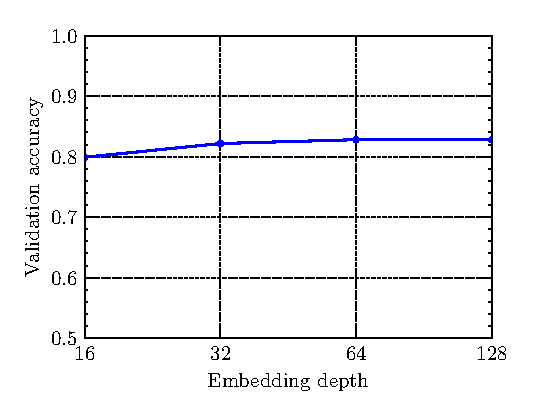
\includegraphics[width=\textwidth]{assets/acc_vs_hyperparam/emb_depth.eps}
        \caption{Accuracy vs. \texttt{d\_model}}
        \label{fig:emd_depth_acc}
    \end{subfigure}
    \hfill
    \begin{subfigure}[b]{0.45\textwidth}
        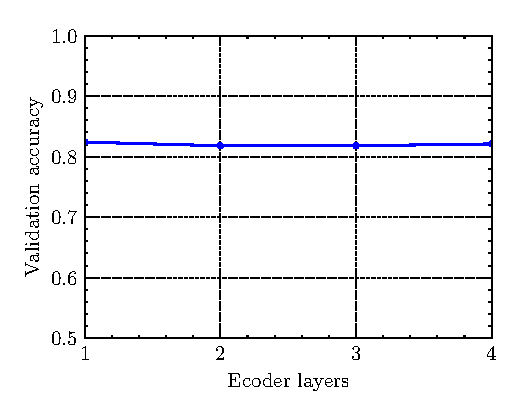
\includegraphics[width=\textwidth]{assets/acc_vs_hyperparam/enc_layer.eps}
        \caption{Accuracy vs. encoder layer count}
        \label{fig:enc_layer_acc}
    \end{subfigure}
    \vfill
    \begin{subfigure}[b]{0.45\textwidth}
        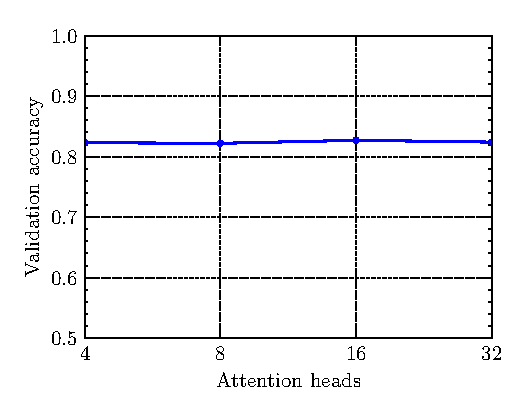
\includegraphics[width=\textwidth]{assets/acc_vs_hyperparam/att_head.eps}
        \caption{Accuracy vs. number of heads}
        \label{fig:att_heads}
    \end{subfigure}
    \hfill
    \begin{subfigure}[b]{0.45\textwidth}
        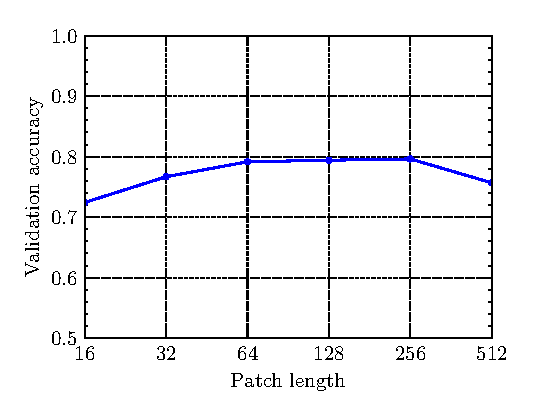
\includegraphics[width=\textwidth]{assets/acc_vs_hyperparam/patch_len.eps}
        \caption{Accuracy vs. patch length}
        \label{fig:patch_len_acc}
    \end{subfigure}
    \vfill
    \begin{subfigure}[b]{0.45\textwidth}
        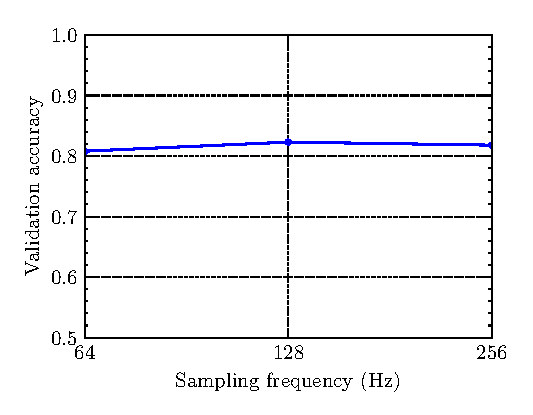
\includegraphics[width=\textwidth]{assets/acc_vs_hyperparam/sampling_freq.eps}
        \caption{Accuracy vs. sampling frequency}
        \label{fig:samp_freq_acc}
    \end{subfigure}
    \hfill
    \begin{subfigure}[b]{0.45\textwidth}
        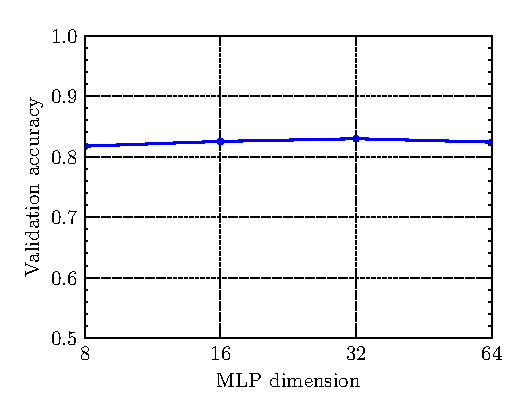
\includegraphics[width=\textwidth]{assets/acc_vs_hyperparam/mlp_dim.eps}
        \caption{Accuracy vs. MLP dimension}
        \label{fig:mlp_dense_layers_acc}
    \end{subfigure}
    \caption{Hyperparameter search results for the vision transformer model}
    \label{fig:model_hyperparameters}
\end{figure}

\begin{table}[ht]
    \centering
    \renewcommand{\arraystretch}{1.2} % Vertical spacing
    \setlength{\arrayrulewidth}{1.5pt} % Thickness of vertical lines
    \caption{Metrics and hyperparameters for vision transformer model}
    \begin{tabularx}{0.7\textwidth}{@{} *1X *1l @{}}
        \toprule
        Metric                          & Value \\\midrule
        Input channel                   & Cz-LER        \\
        Size (\# of weights)            & 31,589        \\
        Sampling frequency              & 128 Hz        \\
        Clip length                     & 30s           \\
        Patch length                    & 64 samples    \\
        Embedding depth ($d_{model}$)   & 64            \\
        \# of attention heads           & 8             \\
        \# of encoder layers            & 1             \\
        MLP dimension                   & 32            \\
        MLP head depth                  & 1             \\
        Output averaging depth          & 3 samples     \\ \bottomrule 
    \end{tabularx}
    \label{tab:model_param}
\end{table}


\newpage
\section{ASIC Accelerator Architecture}
\label{sec:arch}
This section describes and justifies the design of the ASIC accelerator that will run the vision transformer model. It is split into several sections to describe the various aspects
of the accelerator. A high-level overview of the accelerator is shown in Figure \ref{fig:high_level_arch}. As can be seen, it comprises a single Master module responsible for interfacing
with the host system, 64 so-called \ac{cim} modules that perform the actual computation and a shared bus for data and control signals.

\begin{figure}
    \centering
    \includegraphics[width=0.7\textwidth]{assets/high_level_arch.png}
    \caption{High-level architecture of the ASIC accelerator}
    \label{fig:high_level_arch}
\end{figure}

\subsection{Centralized vs. Distributed Architecture}
The first major design aspect of the accelerator is whether to use a centralized or distributed architecture. A centralized architecture has a single compute unit that performs all
operations and a set of relatively large memory banks, while a distributed architecture has multiple compute units, each with their own memory. Of course, linear algebra lends itself
very well to parallelization as each \ac{mac} operation is independent of the others. The centralized architecture is simpler to design, has less overhead and lower area, but is much
slower. It is relatively hard to accurately predict the \ac{ppa} of different architectures before implementation. However, designing a distributed architecture first can be a good
starting point as it can easy be scaled up and down to optimize the design. This is the reason this design uses a distributed architecture.

The design uses 64 \ac{cim} to maximize \ac{pe} utilization of the ASIC as mentioned in Section \ref{sec:sw_hw_co-design}

\subsection{Data and Control Bus}
The data and control bus is a bidirectional bus that connects the Master module and all the \ac{cim} modules. One device may communicate at a time and each is connected to the bus
through tri-state buffers. The bus is 58 bits wide and contains different fields, as summarized in Table \ref{tab:bus_fields}. There are 10 different operations \texttt{Op}, as described
in Appendix \ref{app:bus_ops}. The bus being directly connected to all modules allows for two important features: broadcast and synchronization. There are two types of broadcast: dense
and transpose. Dense broadcast is used to send the same data to all \ac{cim} modules and is used during matrix-matrix multiplications, while transpose broadcast is used to transpose the
matrix (a \ac{cim} holds a row instead of a column, or vice-versa). The \ac{cim}s are autonomous with these operations. They do not need involvement from the Master other than to start
the broadcast. Synchronization is maintained with the \texttt{START\_PISTOL} broadcast, which instructs the \ac{cim}s to go to the next high-level step in their \ac{fsm}.

\begin{table}[ht]
    \centering
    \renewcommand{\arraystretch}{1.2} % Vertical spacing
    \setlength{\arrayrulewidth}{1.5pt} % Thickness of vertical lines
    \caption{Fields of the data and control bus}
    \begin{tabular}{@{} p{1cm}ccc @{}}
        \toprule
        Field           & Width (bits)  & Description \\\midrule
        \texttt{Op}     & 4             & Opcode of the instruction/data \\
        \texttt{ID}     & 6             & ID of the sender or target \ac{cim} \\
        \texttt{Data}   & $3\times16$   & Data (up to 3 $\times$ Q6.10) \\
        \bottomrule
    \end{tabular}
    \label{tab:bus_fields}
\end{table}

\subsection{Master Architecture}
The Master module is responsible for interfacing with the host system. It is a simple module that receives signals from the host microprocessor to start parameter load and start a new
inference. It also interfaces with the external memory holding the parameters and the \ac{adc} in the \ac{eeg} \ac{afe}. It is responsible for directing the \ac{cim} to perform dense
or transpose data broadcasts and for synchronizing their high-level (step-by-step or multi-step) operations.

\subsection{Compute-in-Memory: Architecture}
The \ac{cim} module is the heart of the accelerator. Its architecture is presented in Figure \ref{fig:cim_arch}. It is responsible for performing the actual computation. Each \ac{cim}
module has its own memory for intermediate results and parameters along with control logic and several compute units needed to perform all computation in the model. The \ac{cim} module
is designed to be as autonomous as possible to limit control overhead. It follows the dataflow model of computation, where data is passed from one step of the inference to the next without
Master involvement, unless data needs to be broadcast or transposed across \ac{cim}. The following sections describe different aspects of the \ac{cim} module.
\begin{figure}
    \centering
    \includegraphics[width=0.7\textwidth]{assets/cim_arch.png}
    \caption{Architecture of the Compute-in-Memory module}
    \label{fig:cim_arch}
\end{figure}

\subsection{Compute-in-Memory: Memory}
The \ac{cim} module contains two single-port memory banks: one for intermediate results and one for model weights containing 848 and 528 words, respectively. Having two separate banks
allows for simultaneous read/write to both banks. The memory is generated by ARM's Artisan IP memory compiler and is a 65nm 6T SRAM cell measuring 0.525\si{\mu\square\meter}. It has
an aspect ratio of 4, which, as seen in Figures \ref{fig:mem_area} and \ref{fig:mem_overhead}, provides the lowest overhead for the given capacity. The memories offer single-cycle latency.
They can also be switched into a low-power mode when not in use. Table \ref{tab:mem_metrics} shows various metrics of the memory banks for operation at 1.0V and 25\si{\degreeCelsius}. 

\begin{figure}
    \centering
    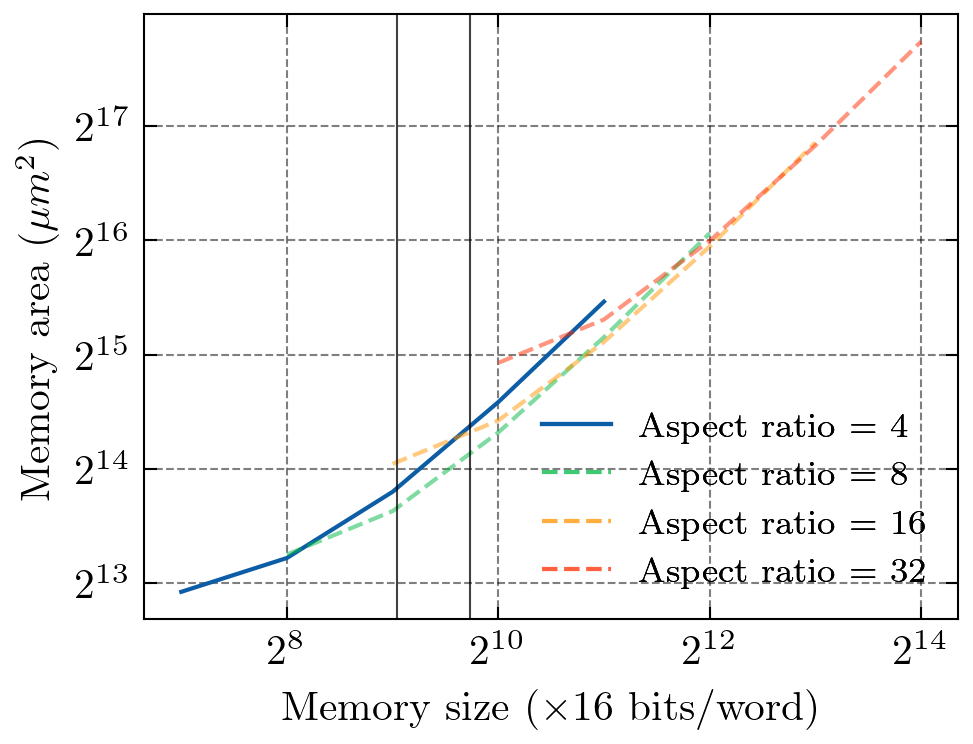
\includegraphics[width=0.7\textwidth]{assets/mem_overhead/mem_area.png}
    \caption{Area of memory banks vs capacity for different aspect ratios}
    \label{fig:mem_area}
\end{figure}
\begin{figure}
    \centering
    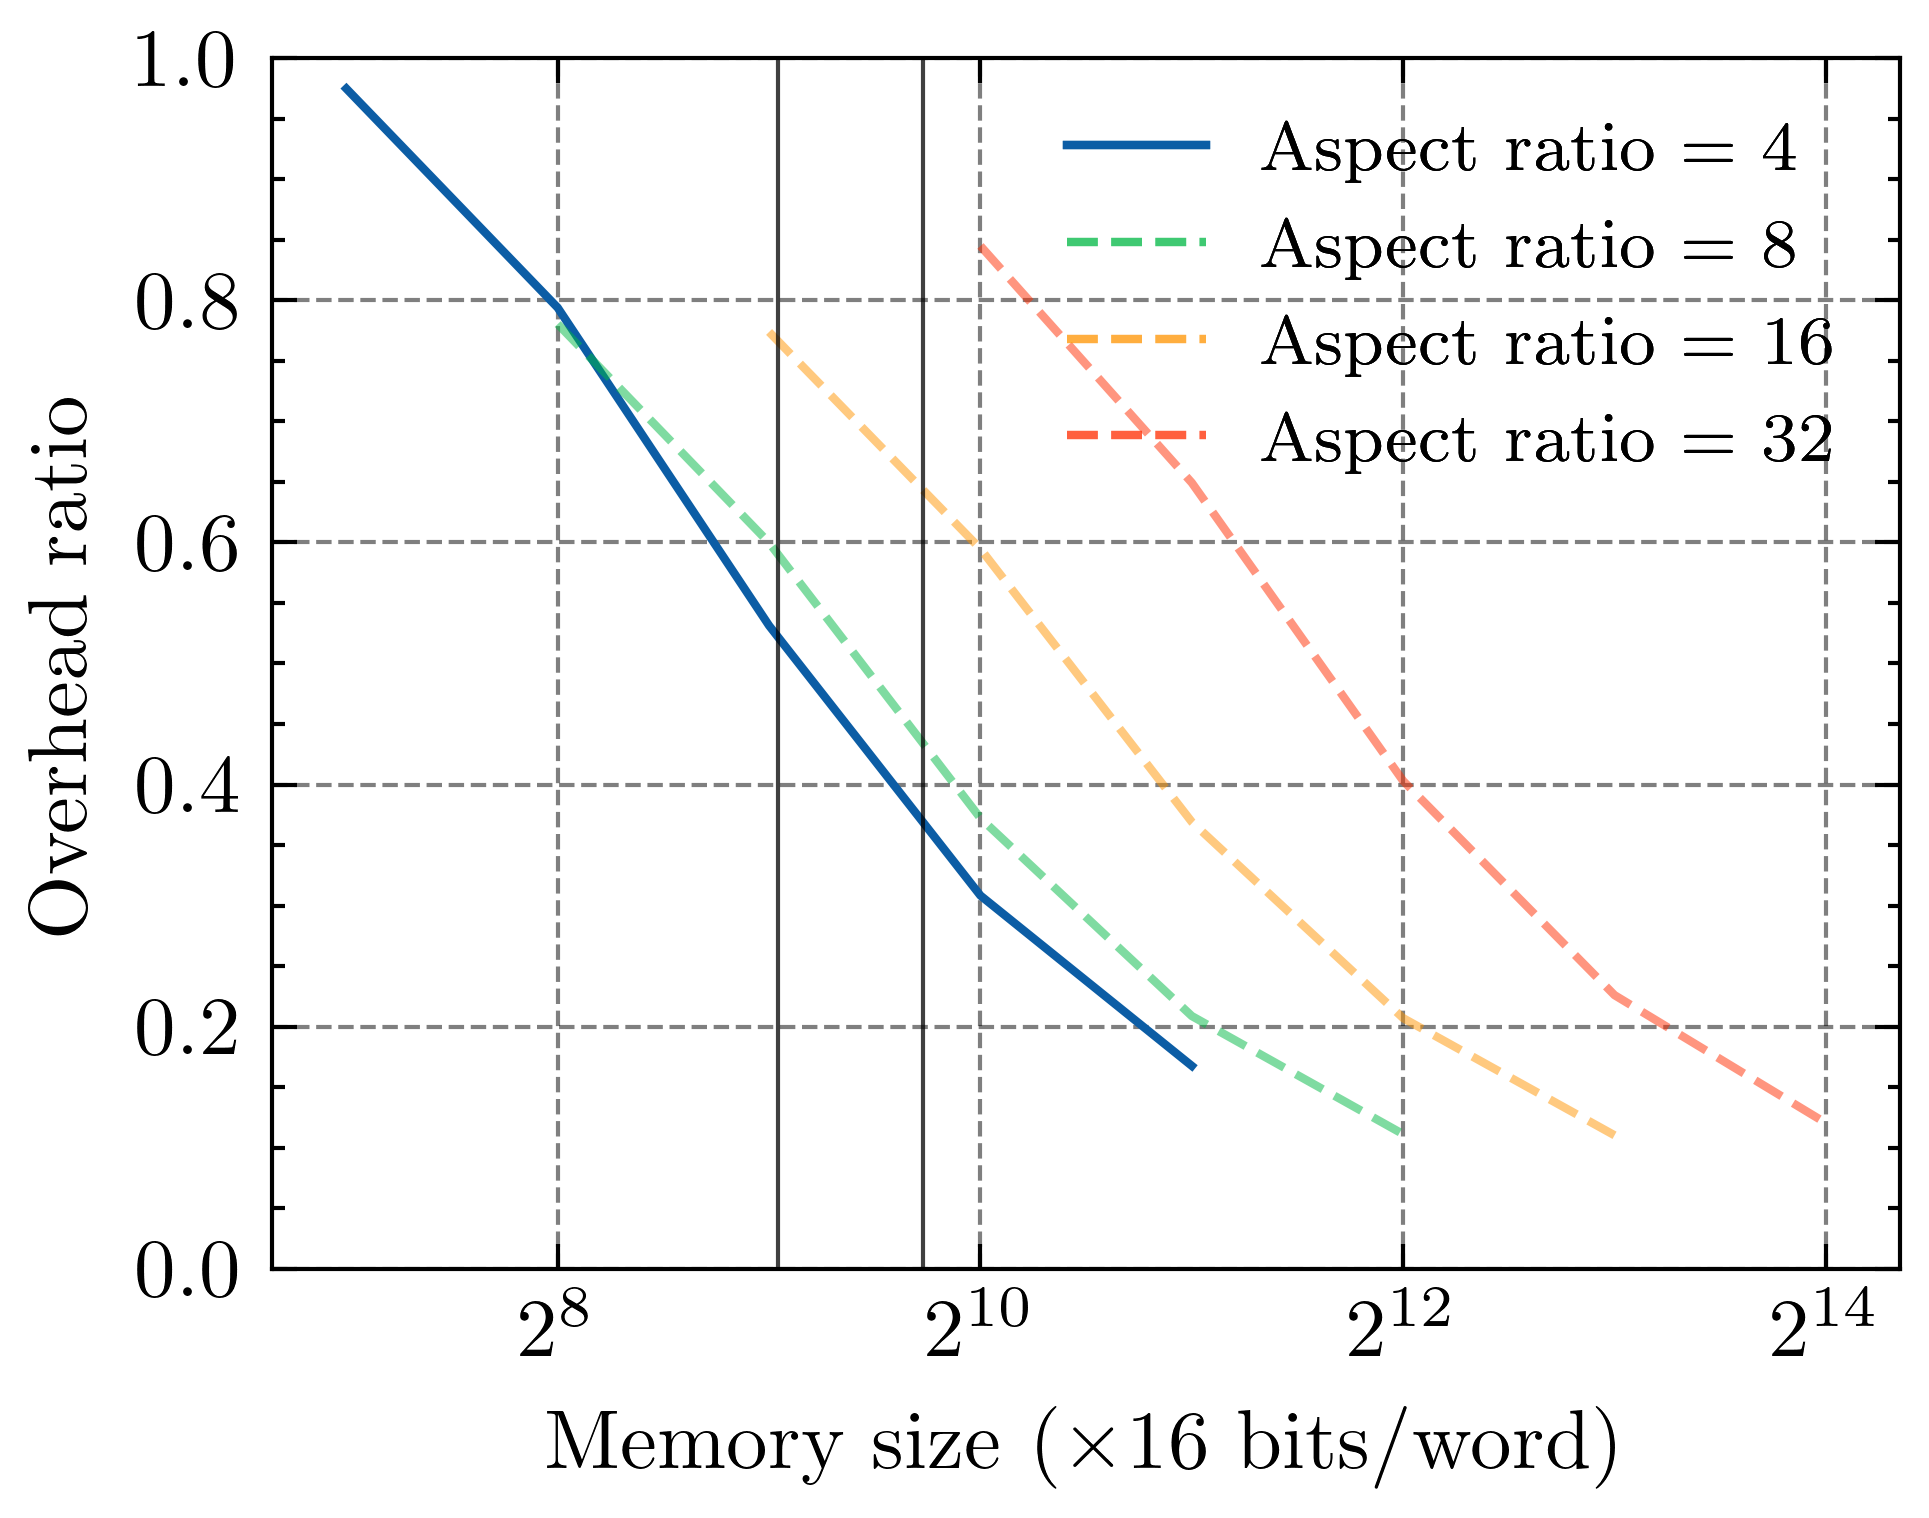
\includegraphics[width=0.7\textwidth]{assets/mem_overhead/mem_overhead.png}
    \caption{Overhead of memory as a fraction of total area for different aspect ratios}
    \label{fig:mem_overhead}
\end{figure}

\begin{table}[ht]
    \centering
    \renewcommand{\arraystretch}{1.2} % Vertical spacing
    \setlength{\arrayrulewidth}{1.5pt} % Thickness of vertical lines
    \caption{Area, leakage power and cycle of the SRAM memory banks}
    \begin{tabular}{@{} p{6cm}ccr @{}}
        \toprule
        Metric                      & 528 words                     & 848 words                     \\\midrule
        Area                        & 16682.54\si{\mu\square\meter} & 22124.25\si{\mu\square\meter} \\
        Leakage (nominal)           & 0.122\si{\milli\watt}         & 0.173\si{\milli\watt}         \\
        Leakage (data retention)    & 0.0754\si{\milli\watt}        & 0.055\si{\milli\watt}         \\
        Cycle time                  & 0.852\si{\nano\second}        & 0.865\si{\nano\second}        \\
        \hline
    \end{tabular}
    \label{tab:mem_metrics}
\end{table}

\subsection{Compute-in-Memory: Fixed-Point Accuracy}
All computation in the \ac{cim} module is done in fixed-point format. The model uses Q22.10 format, which has 22 integer bits (including one sign bit) and 10 fractional bits for 
temporary results internal to the compute modules and Q6.10 for storage. This format was chosen because it significantly reduces the area and power consumption of the accelerator compared
to floating-point format. The fixed-point format is also sufficiently accurate for the model. To determine the accuracy of the fixed-point format, an error study was conducted on the
functional simulation. Using the \texttt{fpm} library, all data operations were performed in fixed-point format. The model was ran on a randomly-selected night of sleep data and the output
was compared to the output of the TensorFlow model and the ground truth. Figure \ref{fig:fixed_point_error} shows the error of the fixed-point format compared to the ground truth as a
function of the number of fractional bits (on a 32-bit fixed-point number). As can be seen, the accuracy peaks at 8 bits of fractional precision, only 1.0\% below the accuracy of the
TensorFlow model (which uses 32-bit floating-point format). We can also notice that accuracy drops significantly starting at 19 fractional bits. This is because some intermediate results
overflow when the numbers have less than 12 integer bits, especially because of operations such as \ac{mac}, softmax and LayerNorm, which accumulate numbers over a length of 64. One
limitation of the \texttt{fpm} library is that it can only represent numbers with a total bit count of 4, 8, 16, 32 or 64 bits, so the ideal number of integer bits cannot precisely be
determined. Although the ideal number of fractional bits is 8, the design uses 10 fractional bits to provide a small margin of error and guard against divides by zero with other input nights.

\begin{figure}
    \centering
    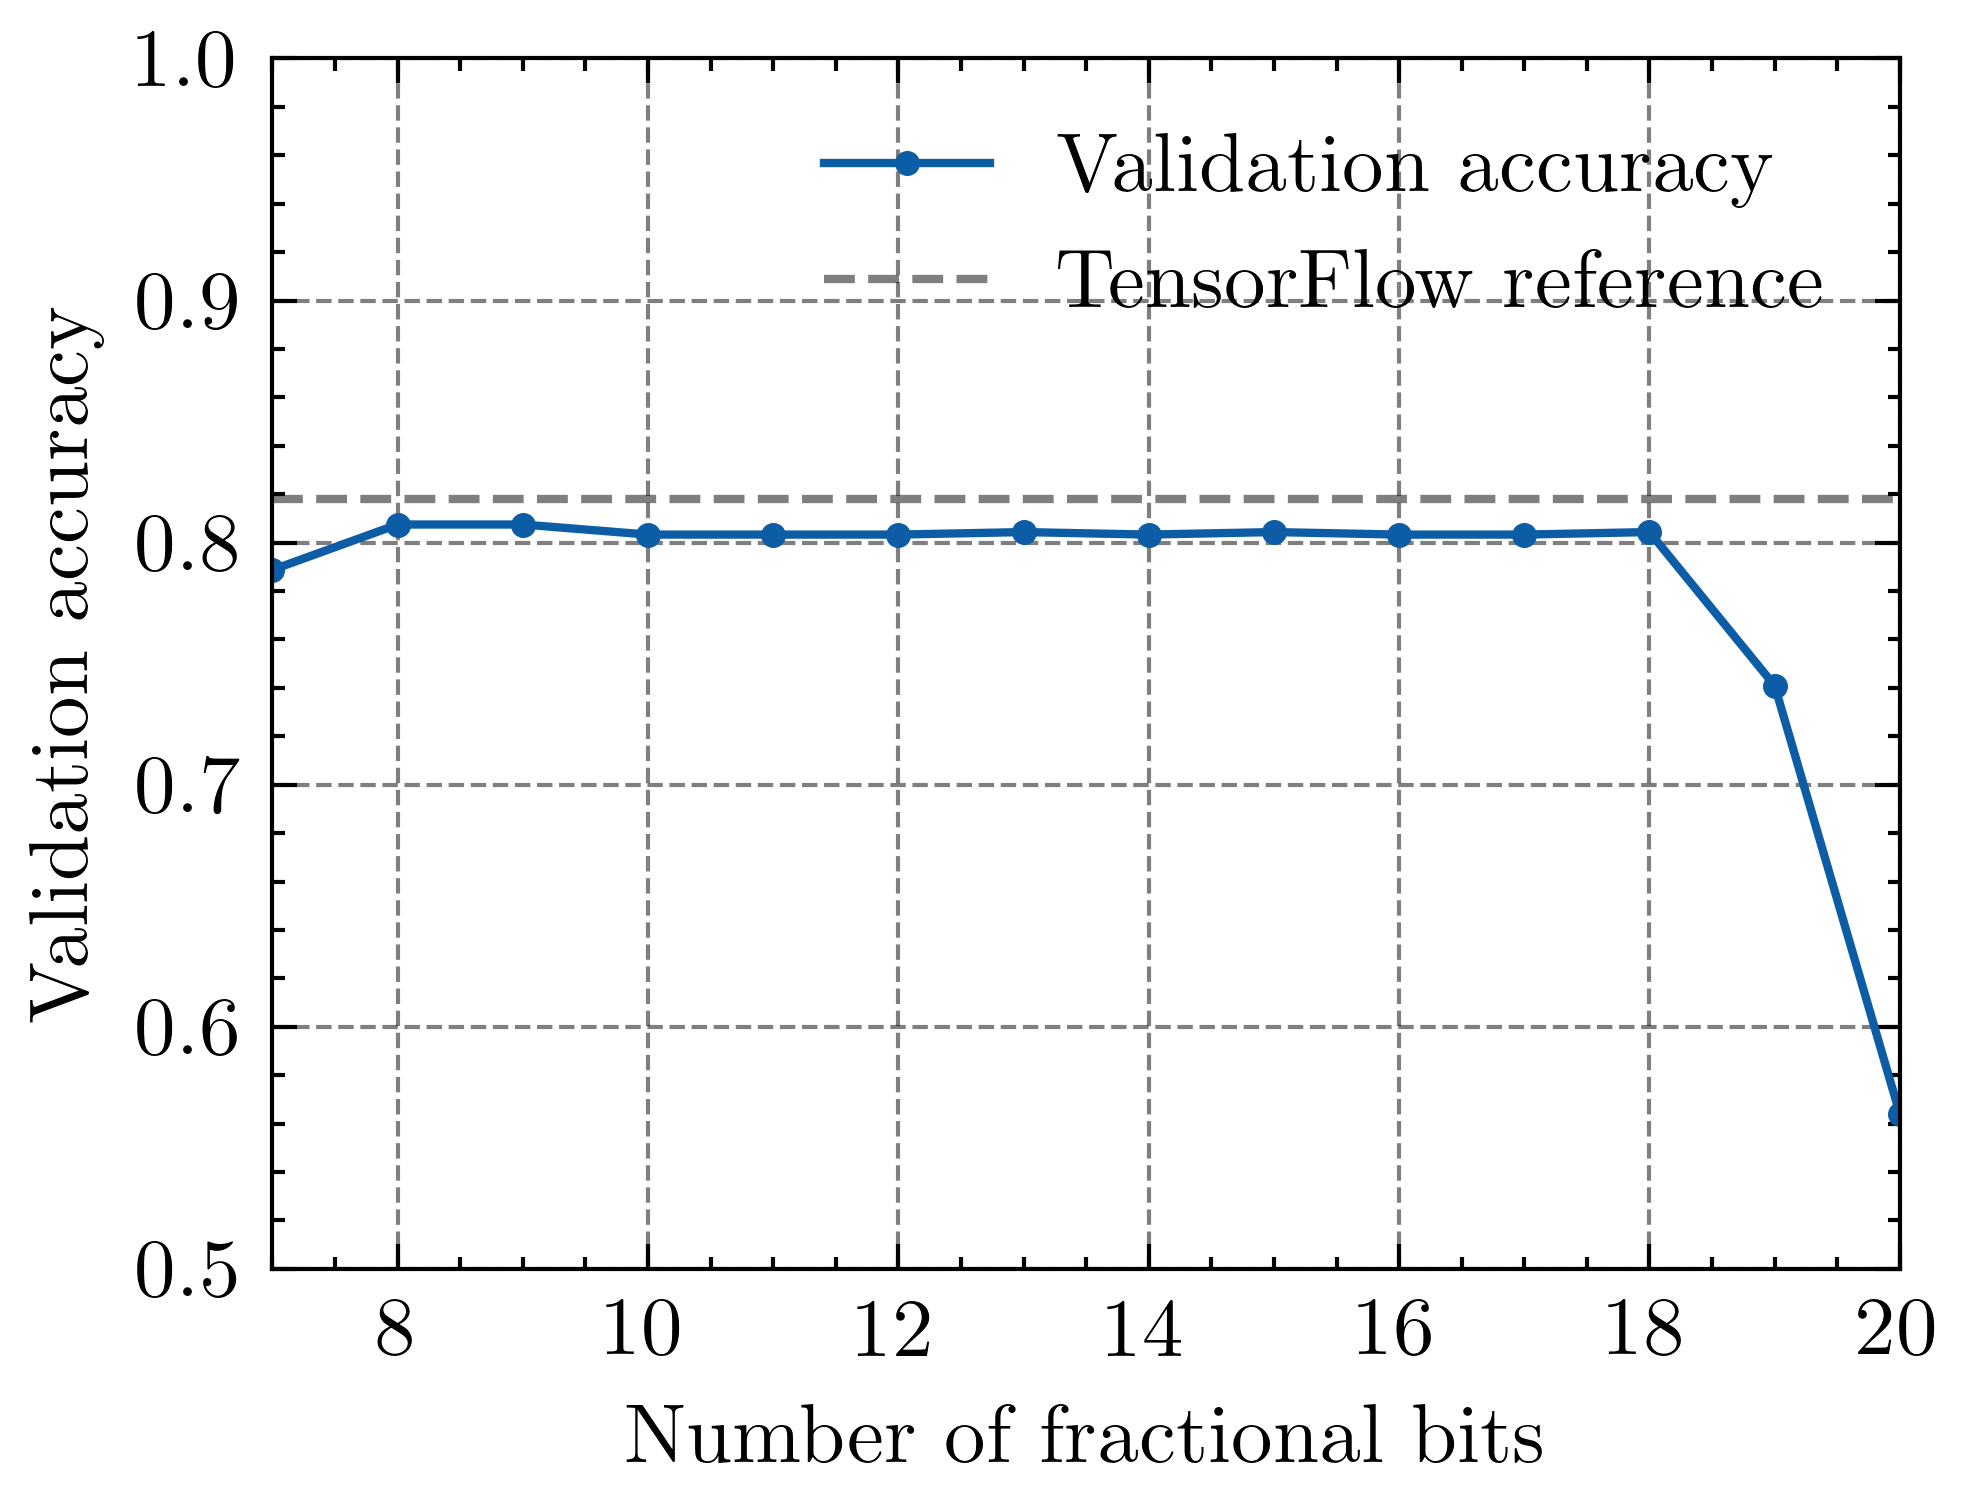
\includegraphics[width=0.7\textwidth]{assets/fixed_point_acc/fixed_point_acc.png}
    \caption{Model accuracy vs number of fractional bits in fixed-point format}
    \label{fig:fixed_point_error}
\end{figure}

\subsection{Compute-in-Memory: Compute Modules}
\label{sec:arch_compute}
This section describes the design and performance metrics of the various compute \ac{ip} modules used in the design. Each is custom-designed for this project. Each module works with signed
(2's complement) fixed-point representation. To avoid overflow, the modules use internal temporary variables of fixed-point format Q22.10. Table \ref{tab:compute_modules} shows the performance
metrics of the compute modules. The working principles of each modules is described briefly in subsequent sections.

\begin{table}[ht]
    \centering
    \renewcommand{\arraystretch}{1.2} % Vertical spacing
    \setlength{\arrayrulewidth}{1.5pt} % Thickness of vertical lines
    \caption{Performance metrics of the compute modules}
    \begin{tabular}{@{} p{2.5cm}ccccc @{}}
        \toprule
        Module                  & Area                          & Cycle/op  & Energy/op                 & Leakage power         & $F_{max}$ \\\midrule
        Adder                   & 450.4\si{\mu\square\meter}    & 1         & 0.99\si{\pico\joule}      & 11.87\si{\mu\watt}    & 6.67\si{\giga\hertz}  \\
        Multiplier              & 3535.2\si{\mu\square\meter}   & 1         & 7.05\si{\pico\joule}      & 90.50\si{\mu\watt}    & 1.59\si{\giga\hertz}  \\
        Divider                 & 1719.9\si{\mu\square\meter}   & 35        & 23.44\si{\pico\joule}     & 34.56\si{\mu\watt}    & 1.11\si{\giga\hertz}  \\
        Exponential             & 2442.2\si{\mu\square\meter}   & 24        & 62.73\si{\pico\joule}     & 47.10\si{\mu\watt}    & 7.14\si{\giga\hertz}  \\
        Square Root             & 1325.2\si{\mu\square\meter}   & 21        & 18.32\si{\pico\joule}     & 26.30\si{\mu\watt}    & 0.758\si{\giga\hertz} \\
        MAC\footnotemark[1]     &                               & 386       & 820.20\si{\pico\joule}    &                       &                       \\
        MAC\footnotemark[2]     & 3129.8\si{\mu\square\meter}   & 391       & 839.32\si{\pico\joule}    & 69.40\si{\pico\joule} & 2.17\si{\giga\hertz}  \\
        MAC\footnotemark[3]     &                               & 456       & 941.68\si{\pico\joule}    &                       &                       \\
        Softmax                 & 2341.1\si{\mu\square\meter}   & 2024      & 1972.5\si{\pico\joule}    & 51.47\si{\mu\watt}    & 1.20\si{\giga\hertz}  \\
        LayerNorm               & 3836.89\si{\mu\square\meter}  & 1469+494  & 1705.7\si{\pico\joule}    & 78.39\si{\mu\watt}    & 0.877\si{\giga\hertz} \\
        \bottomrule
        Total                   & 18780.69\si{\mu\square\meter} & N/A       & N/A                       & 409.59\si{\mu\watt}   & 0.758\si{\giga\hertz} \\
        \hline
    \end{tabular}
    \begin{minipage}{\textwidth}
        \noindent\hspace*{1cm}\textsuperscript{1} No activation function applied\\
        \noindent\hspace*{1cm}\textsuperscript{2} Linear activation function applied\\
        \noindent\hspace*{1cm}\textsuperscript{3} Swish activation function applied
    \end{minipage}
    \label{tab:compute_modules}
\end{table}

Note that all measurement in Table \ref{tab:compute_modules} are given for standard 65nm \ac{tsmc} process. To determine these metrics, the following methodology was used with Synopsys
Design Compiler 2017.09 running on UofT's EECG cluster:
\begin{itemize}
    \item Area: Synthesis with the area optimization effort set to \texttt{high}, and the area was extracted from the \texttt{report\_area} command report.
    \item Cycle/op: The latency was observed when running a single operation on a pre-synthesis simulation.
    \item Energy/op: A single-instance testbench running 1000 operations was designed, and a \texttt{.saif} file was generated from the \ac{vcd} dump file of the testbench
    using Synopsys' \texttt{vcd2saif} utility. This provides an average activity factor for each node, yielding an accuracy that is adequate for this discussion. The energy
    per operation was calculated by normalizing the total energy used by the number of operations performed in the testbench.
    \item Leakage power: Synthesis with the power optimization effort set to \texttt{high}, and the leakage power was extracted from the \texttt{report\_power} command report.
    \item $F_{max}$: The \texttt{report\_timing} command was used to determine the maximum frequency of the design.
\end{itemize}

It must be noted that the measurements for all composite compute units (i.e. units that make use of shared resources) \textit{exclude} the area/power/etc. of the shared resources.
Including them would result in misleadingly high figures, given that they are explictly designed to share resources. The total area of the \ac{cim} provides figures more representative
of this integration.

\subsubsection{Adder}
The adder is a single-cycle, combinational module that adds two fixed-point numbers. It uses a ripple-carry adder architecture. The adder has a latency of 1 cycle, which simplifies the
logic that uses it. It also provides an overflow flag. To reduce dynamic power consumption, the adder only updates its output when the \texttt{refresh} signal is high.

\subsubsection{Multiplier}
The multiplier is very similar to the adder. One difference is that it uses Gaussian rounding (also known as banker's rounding). This method rounds up or down in an alternating fashion.
This reduces the bias in the output that is commonly observed with standard rounding methods, which is particularly important in \ac{mac} or LayerNorm operations where the error can
accumulate. The multiplier also has a latency of 1 cycle and provides an overflow flag. Like the adder, the multiplier only updates its output when the \texttt{refresh} signal is high.

\subsubsection{Divider}
The divider is more complicated than the adder and multiplier. It performs bit-wise long-division and has a latency of $N+Q+3$ cycles, where $N$ is the number of integer bits and $Q$ is
the number of fractional bits. The divider also provides flags for overflow and divide-by-zero and done/busy status signals. The module start division on an active-high pulse of the \texttt{start}
signal and provides the result when the \texttt{done} signal is high.

\subsubsection{Exponential}
The exponential module computes the natural exponential, $e^{x}$, of a fixed-point number $x$. It uses a combination of the identities of exponentials and a Taylor series approximation around
zero to compute the exponential. Specifically, the module transforms the exponential as such:
\begin{equation}
    e^{x} = 2^{\frac{x}{\ln(e)}} = 2^{z} = 2^{\lfloor{z}\rfloor}2^{z-\lfloor{z}\rfloor}
    \label{eq:exp_transform}
\end{equation}
The module can then easily compute $2^{\lfloor{z}\rfloor}$ as an inexpensive bit-shift operation and $2^{z-\lfloor{z}\rfloor}$ as a Taylor series approximation. To determine a reasonable
number of terms to use for the Taylor series expansion, an accuracy study was ran. Figure \ref{fig:exp_error} shows the relative error of the exponential module as a function of the order
of the Taylor series expansion for both fixed-point (Q22.10) approximation and float (64-bit) approximation. As can be seen, the error decreases with an increase in the order of the expansion.
However, for the fixed-point approximation, it converges to a minimum error of 0.992\%. This is because the quantization of fixed-point dominates the Taylor series error. Therefore, using
a 3rd order Tarlor series expansion to approximate the exponential function is a good balance between accuracy and latency/energy. Note that this error was measured over the input range of
[-4, 4]. According to the functional simulation, this corresponds to roughly $\pm3$ standard deviations from the mean of inputs to the exponential function. To further speed up the computation,
the exponential module uses a lookup table to store the Taylor series coefficients as well as $1/ln(e)$. To reduce area, the exponential module does not instantiate its own adder and multiplier
modules. Rather, it accesses the adder and multiplier modules in the \ac{cim} module shared with other compute units. The latency is 24 cycles.

\begin{figure}
    \centering
    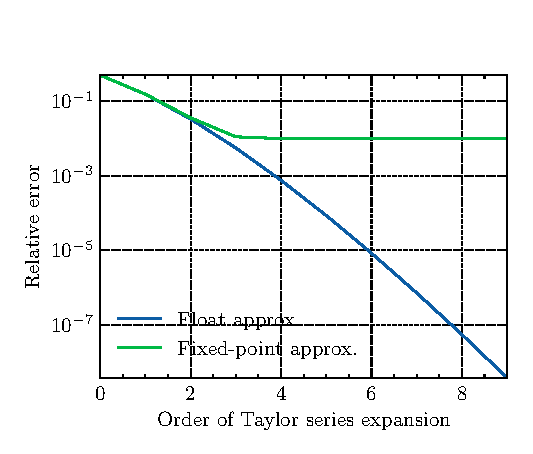
\includegraphics[width=0.7\textwidth]{assets/exp_approx_error/exp_approx_error.eps}
    \caption{Approximation error of the exponential vs Taylor series expansion order}
    \label{fig:exp_error}
\end{figure}

\subsubsection{Square Root}
The square root module computes the square root of a fixed-point number using an iterative algortihm. It has a latency of $(N+Q)//2+1$ cycles, where $//$ denotes integer division. The module 
provides flags for overflow and negative radicand and \texttt{start}/\texttt{busy}/\texttt{done} signals. The module starts computation on an active-high pulse of the \texttt{start} signal and provides the result when 
the \texttt{done} signal is high.

\subsubsection{Multiply-Accumulate}
The \ac{mac} module performs a vector dot-product for a given pair of base addresses for the data and length of the vector and applies a selectable activation function to the result. Similarly
to the exponential module, it uses shared adder, multiplier, divider and exponential modules in the \ac{cim} module. It can implement three activation functions: none, linear and Swish. As
reported by Ramachandran \textit{et al}, Swish is similar to SiLU and helps resolve the vanishing gradient problem in backpropagation, leading to a higher accuracy for a given number of training
epochs \cite{ramachandran2017searching}. For a nominal length of 64 (which corresponds to the embedding depth of the model, a very common value for matrix dimensions in the model) and Q22.10 format,
the latencies are 386, 391 and 456, respectively. Note that, although the Swish activation function comprises a divider operation, the \ac{mac} compute latency can still be kept fairly short because
the divisor is the same for all elements. The module can thus perform the division once and multiply by the inverse, which is a single-cycle operation. Finally, the \ac{mac} module can be directed
to choose the second vector from weights or intermediate results memory.

\subsubsection{Softmax}
The softmax module computes the softmax function of a vector of fixed-point numbers. Similarly to the \ac{mac} module, it uses shared adder, mulitplier, divider and exponential modules and 
provides \texttt{busy} and \texttt{done} signals. For a 64-element Q22.10 vector, the latency is 2024 cycles. This is significantly longer than other vector compute modules such as the \ac{mac}
because, in the softmax operation, each element is exponantiated individually.

\subsubsection{LayerNorm}
The final compute module is the LayerNorm module. It computes the Layer Normalization of a vector of fixed-point numbers. As described in section \ref{sec:vision_transformer}, the LayerNorm 
operation consists of a normalization of the vector on the horizontal dimension followed by scaling and shifting using learnable parameters on the vertical dimension. Because each \ac{cim} 
module stores one vector at a time, the LayerNorm operation must be separated into two stages with a matrix transpose broadcast between the two. The latency for the first half is 1469 cycles 
and the latency for the second half is 494 cycles. The module provides \texttt{busy} and \texttt{done} signals and is controlled with a \texttt{half-select} and \texttt{start} pulse signals.
Because the length of the vector is constrained to be a power of two, the module uses bit-shifting instead of division for the normalization operation to decrease latency and energy per operation.

\subsection{Clock Gating}
This design makes use of clock gating, which is a technique to reduce dynamic power consumption by disabling the clock signal to modules that are not in use. This is handled automatically by
the Synopsys Design Compiler tool.


\subsection{A Note About Software-Hardware Co-Design}
\label{sec:sw_hw_co-design}
To maximize utilization (and thus time- and physical efficiency) and reduce latency (thus reducing inference energy), the model and accelerator were designed together. An example
of this software-hardware co-design concerns the number of \ac{cim} in the accelerator. Most weights and intermediate results matrices have at least one dimension that is 61 (number
of patches + classification token) or 64 (embedding depth of the model). With 64 \ac{cim}s, all vector operations can be computed simulatenously, avoiding extra overhead for control
and data movement while limiting the amount of unused silicon. This is the main reason behind the choice of 64 samples for the patch length, which also yields 60 patches per sleep
epoch. Furthermore, the embedding depth of the model is a power of 2, meaning that all divisions (such as in the LayerNorm) with this number can be accomplished with inexpensive bit shifts.

\newpage
\section{Results: Evaluation of Performance Metrics}
\label{sec:results}
This presents and discusses the most salient aggregate high-level results of the model and hardware design shown in Table \ref{tab:high_level_results}.
It can be seen that the model meets the requirements summarized in Table \ref{tab:design_goals}. Indeed, the model size (63.18\si{\kilo\byte}) is below the
125\si{\kilo\byte} target, and the accuracy (82.9\%) is higher than the 80\% target. It is also nearly $32\times$ smaller than the smallest state-of-the-art
model for automatic sleep staging presented by Eldele \textit{et al.}, which has 500000 32-bit floating point parameters \cite{eldele2021attention}.

The ASIC accelerator meets some of the requirements. The inference latency (6.97\si{\milli\second}) is well below the maximum allowed latency of 3\si{\second}.
The \ac{pe} utilization (50.8\%) of the accelerator suggests that there is non-negligible time overhead (mostly from inter-\ac{cim} communication) that could be
reduced in future work. The toral area is 3.86\si{\square\milli\meter}, which is above the target of 1.5\si{\square\milli\meter}. The effective power is below the
ceiling of 5\si{\milli\watt}.

The effective total power considers the effects of power gating, which is a common technique used in modern processors to reduce power consumption. The idea
is to turn off power to the ASIC accelerator when it is not in use through one or more low-side \ac{nmos} (known as a ``sleep transistor''). Investigating this
technique for 65nm \ac{cmos} technology, Sathanur \textit{et al.} found that leakage power can be reduced by up to 95\% using power gating \cite{sathanur2008quantifying}.
The effective total power is calculated as the sum of the average dynamic power from inference energy and the leakage power pro-rated with power gating. It assumes a
sleep epoch duration of 30\si{second}. The average dynamic power is computed for an inference with the techniques of analyzing a \ac{vcd} file as described in 
Section \ref{sec:arch}.

With an inference latency of 6.97\si{\milli\second} and a sleep epoch duration of 30\si{\second}, the ASIC accelerator only runs for 0.0232\% of the time, meaning
that the effective leakage power is reduced by up to 94.98\%, reducing the effective leakage power to 2.947\si{\milli\watt}. The accelerator consumes a total of
63.07\si{\milli\watt} during inference, which is reduced to 3.046\si{\milli\watt} with power gating. The energy per inference is 433.29\si{\micro\joule}. 

\begin{table}[ht]
    \centering
    \renewcommand{\arraystretch}{1.2} % Vertical spacing
    \setlength{\arrayrulewidth}{1.5pt} % Thickness of vertical lines
    \caption{Principal results of the model and hardware design}
    \begin{tabularx}{0.8\textwidth}{Xlc}
        \toprule
        Metric                      & Value                         & Meets requirement? \\\midrule
        31-fold accuracy            & 82.9\%                        & Yes   \\
        \# of parameters            & 31,589                        & Yes   \\
        Size                        & 63.18\si{\kilo\byte}          & Yes   \\ \bottomrule 
        %%%%%%%%%%%%%%%%%%%%%%
        Inference latency           & 6.87\si{\milli\second}        & Yes   \\
        Area                        & 3.86\si{\square\milli\meter}  & No    \\
        \ac{pe} utilization         & 50.8\%                        & N/A   \\
        Leakage power               & 56.48\si{\milli\watt}         & N/A   \\
        Average dynamic power       & 6.59\si{\milli\watt}          & N/A   \\
        Effective total power       & 3.046\si{\milli\watt}         & Yes   \\
        Energy/inference            & 433.29\si{\micro\joule}       & N/A   \\
        $F_{Max}$                   & 758\si{\mega\hertz}           & Yes   \\ \bottomrule
    \end{tabularx}
    \label{tab:high_level_results}
\end{table}

\newpage
\section{Results Analysis \& Future Work}
Based on the design and results discussions of Sections \ref{sec:vision_transformer}, \ref{sec:arch} and \ref{sec:results}, the design as presented is not recommended to be used
further for the sleep staging earpiece project. This section discusses suggested improvements and future work to maximize the utility of this project. Tables \ref{tab:model_improvements}
and \ref{tab:hw_improvements} summarize the suggested improvements and attempts to quantify their benefits wherever reasonable.

\subsection{Vision Transformer Model Improvements}
The vision transformer can be improved in different ways, from training to simplification of operations. Firstly, the model could be pre-trained on the \ac{stages} dataset
\cite{zhang2018national}, which contains PSG recordings from 1500 patients, significantly more than the 62 nights available in the dataset (\ac{mass} SS3 \cite{SP3/9MYUCS_2022})
currently used. Although \ac{mass} is widely used for model benchmarking, it is worthwhile to try pre-training the model on \ac{stages} and perform transfer learning and k-fold
validation on the \ac{mass} dataset. In addition, the model should be trained and validated on the Expanded Sleep-EDF dataset, which is the most widely used dataset in the literature
\cite{physiobank2000physionet}. Once the annotated \ac{eeg} data measured in-ear is available, the model will need to be trained on the new dataset. Weight pruning could further
reduce the size of the model. Pruning consists of eliminating a subset of weights to reduce model size and compute with minimal loss of accuracy at the cost of more complicated
control logic. In some cases, pruning may also increase accuracy. Indeed, Chen \textit{et al.} applied 50\% pruning on DeiT-Small, a vision transformer model, and observed a 0.28\%
accuracy boost. Furthemore, it would be beneficial to eliminate the $\gamma$ and $\beta$ learned parameters used to scale and shift the normalized values in the LayerNorm steps. These
add six broadcast transpose operations to the inference, which represents 9.69\% of the total inference time and effective total power. Finally, it would be beneficial to explore
an architecture that uses more than one \ac{eeg} electrode or different input signals such as heartrate or temperature as a means of increasing accuracy further. Most models in the
literature use 2-5 electrodes \cite{zhuang2022intelligent, phan2021xsleepnet}. This improvement is particularly relevant given the earbud form factor which can accommodate multiple
contact eletrodes and other biosignals. Indeed, in the summer of 2023, Apple was granted a patent for an in-ear ``biosignal sensing device'' covered with different types of electrodes
such as \ac{emg}, \ac{eog}, \ac{ecg}, \ac{bvp} and \ac{gsr} \cite{apple2023biosignal}. This modification will undoubtedly increase the area and latency, and an evaluation of whether the
potential increase in accuracy is worth it should be performed.

\begin{table}[ht]
    \centering
    \renewcommand{\arraystretch}{1.2} % Vertical spacing
    \setlength{\arrayrulewidth}{1.5pt} % Thickness of vertical lines
    \caption{Suggested improvements to the model and their potential benefits}
    \begin{tabular}{@{} p{7cm}ccc @{}}
        \toprule
        Improvement                         & Accuracy $\Delta$ & Latency $\Delta$                  & Area $\Delta$ \\\midrule
        \ac{stages} and Expanded Sleep-EDF  & Unknown           & No change                         & No change     \\
        Weight pruning                      & Unknown           & $\downarrow$                      & $\downarrow$  \\ 
        $\gamma$ and $\beta$ elimination    & Unknown           & 0.666\si{\milli\second}/-9.69\%   & No change     \\
        Additional channels and electrodes  & $\uparrow$        & $\uparrow$                        & $\uparrow$    \\\bottomrule
    \end{tabular}
    \label{tab:model_improvements}
\end{table}

It would also be important to rewrite the model in efficient C code and run on a microcontroller to determine how far from targets a firmware approach might be. Multiple authors have 
published relevant work for the RISC-V \ac{isa}, such as an extension to handle vector operations \cite{perotti2022new} or compilation support for a RISC-V + CGRA heteregenous architecture
\cite{lingRISC-V-CGRA}. Running the model on a microprocessor would save the significant development and verification effort of an ASIC accelerator and allow for a more flexible design since
the model could be changed with a firmware update. However, the power consumption and area of a vector- or CGRA-augmented microcontroller might be higher than the ASIC accelerator.

\subsection{Accelerator ASIC Improvements}
The bulk of suggested improvements to this project are in the hardware design. It can be made much smaller and more power-efficient. The first recommendation is to use a centralized
architecture for the memory. This will save significant area and leakage power mainly from the reduction of memory overhead and deduplication of area dedicated to storing addresses.
Specifically, for centralizing memory alone, Figure \ref{fig:mem_overhead} shows that, using two banks holding 15,794 words (enough to contain the full model) and 4 banks for the
intermediate results will reduce the memory overhead from 49.5\% (weighted average of the overhead of the parameters memory and the weights memory in the current \ac{cim} architecture)
to 12.0\%, saving 0.931\si{\square\milli\meter}. The total leakage will also decrease by 13.75\si{\milli\watt}. Centralizing the memory will also slightly reduce the inference latency
since some compute elements that operate on two intermediate results, such as some configurations of the \ac{mac} will be able to load the data in parallel. However, this reduction is
expected to be small.

The second recommendation is to use a centralized compute architecture with a single instance of each of the compute elements of Section \ref{sec:arch_compute}. According to Table
\ref{tab:compute_modules}, this will save 1.183\si{\square\milli\meter} of area and 25.80\si{\milli\watt} of leakage power. The dynamic power will also decrease slightly due to reduction
in wiring, although an exact figure is hard to estimate without an implemented design. Although inference time will increase, it will remain far under the requirement of 3s. In fact, the
inference time is expected to be less than 64 times longer than the distributed architecture. Indeed, as mentionned in Section \ref{sec:results}, the \ac{cim} spends roughly 50.8\% percent
of its time in compute. The rest is mainly data broadcast. In data broadcast, the majority of the time (4/7 cycles) is spent waiting for data from the single-port memory. With the
centralized memory banks and a careful addressing scheme, the inference time is expected to increase by $64\times(1-0.508*4/7) = 45.42\times$ or 0.312\si{\second}.

The complete centralization of the memory and compute will eliminate the need for the bus. This will save area and power, although the exact amount is hard to estimate without an implemented
design. Finally, it may be interesting to explore the impact of using a different Q format for the weights and intermediate results at different layers in the model. The current design uses
a constant Q6.10 format for stored data. It may be possible to use fewer bits overall if the Q format can be changed during inference for layers that are known to produce large numbers. This
can save storage area and shrink the compute units; however, it will increase the complexity of the control logic and require storing the Q format to use for each layer. The net impact is 
hard to estimate without a design, and is expected to be fairly small so this recommendation should not be prioritized. For this, the functional simulation of the accelerator should be extended
to perform the study. Shifting away from the \texttt{fpm} library to a more flexible fixed-point library or writing one from scratch to properly emulate non-powers-of-two bitwidths will be
necessary to implement this change.

A key insight from Section \ref{sec:results} is that the leakage power represents 96.7\% of the effective power consumption. A key factor to reducing effective power consumption is power gating
agressiveness. To reduce effective power consumption further and extend battery life of the final device, the power gating investigation of \cite{sathanur2008quantifying} should be extended to
further reduce leakage, perhaps by cascoding sleep transistors or adjusting their body bias to shift their threshold voltage and reduce subthreshold leakage. Stacking transistors will reduce
$f_{Max}$ and increase dynamic energy given the increase in capacitance, but given that both these metrics are well below their constraints, this is acceptable. Cascoding sleep transistors will
also increase area, although this is expected to a minor increase.

\begin{table}[ht]
    \centering
    \renewcommand{\arraystretch}{1.2} % Vertical spacing
    \setlength{\arrayrulewidth}{1.5pt} % Thickness of vertical lines
    \caption{Suggested improvements to the ASIC accelerator and their potential benefits}
    \begin{tabular}{@{} p{3.75cm}cccc @{}}
        \toprule
        Improvement         & Dyn. energy $\Delta$      & Leakage $\Delta$          & Latency $\Delta$      & Area $\Delta$                     \\\midrule
        Centralized memory  & Slight $\downarrow$       & -13.75 \si{\milli\watt}   & Slight $\downarrow$   & -0.931\si{\square\milli\meter}    \\
        Centralized compute & Slight $\downarrow$       & -25.80\si{\milli\watt}    & +0.305\si{\second}    & -1.183\si{\square\milli\meter}    \\
        Bus elimination     & Slight $\downarrow$       & Slight $\downarrow$       & No change             & Slight $\downarrow$               \\
        Optimize Q format   & Indeterminate             & Indeterminate             & Indeterminate         & Indeterminate                     \\
        Power gating        & Slight $\uparrow$         & Significant $\downarrow$  & Slight $\uparrow$     & Slight $\uparrow$                 \\\bottomrule
    \end{tabular}
    \label{tab:hw_improvements}
\end{table}

With the quantified suggested improvements, the leakage power of the ASIC would be reduced from 56.48\si{\milli\watt} to 16.93\si{\milli\watt}. Ignoring improvements to power gating,
this reduces the effective power consumption from 3.046 \si{\milli\watt} to 0.848\si{\milli\watt}, a 72.2\% reduction. The area would decrease from 3.86\si{\square\milli\meter} to 
1.746\si{\square\milli\meter}, a 54.8\% reduction, which brings the total area to just under the objective of 2\si{\square\milli\meter}.

Section \ref{sec:results} has shown that the current design is not suitable for the sleep staging earpiece project as is. However, there is a clear path forward to designing an AI accelerator
with significantly reduced power consumption and area, which are the two most important metrics for the earpiece project.

\newpage
\section{Conclusion}
\label{ref:conclusion}
This thesis has presented a vision transformer-based model for automatic sleep staging and an ASIC accelerator to run the model. This work is part of a larger project aimed at developing an 
in-ear device capable of acoustic neuromodulation to treat insomnia, which requires live, accurate and practical sleep staging. The model achieved 82.9\% accuracy on the MASS SS3 dataset using
a single \ac{eeg} input and has a size of 31,589 parameters. The ASIC accelerator consumes 3.046\si{\milli\watt} on average, has an area of 3.86\si{\square\milli\watt} and an inference latency
of 6.97ms. The results show that performing sleep staging in-ear is not only possible but also practical. The model meets all the requirements summarized in Table \ref{tab:design_goals}, except
for the area of the accelerator. Future work should focus on reducing the power consumption and area of the accelerator. Centralizing compute and memory can reduce power consumption and area by
72.2\% and 54.8\%, respectively. It is also advised to investigate running the model on a RISC-V processor with vector extension or CGRA add-on for additional flexibility and decreased development
risk and timeline.

\newpage

% Bibliography
\AtNextBibliography{\footnotesize}
\printbibliography[heading=bibintoc]
\newpage

% Appendices
\appendix
\section{Codebase Statistics}
It may be interesting to the reader to appreciate the size of the codebase needed to develop a project of similar scale. The code for this project is available 
in my \href{https://github.com/TristanRobitaille/engsci-thesis}{GitHub repository}. The following table provides a breakdown of the number of lines of code in the project.

\begin{table}[ht]
    \centering
    \renewcommand{\arraystretch}{1.2} % Vertical spacing
    \setlength{\arrayrulewidth}{1.5pt} % Thickness of vertical lines
    \caption{Line and file count per file type in the codebase.}
    \begin{tabular}{@{} p{4cm}cccr @{}}
        \toprule
        File type       & File count    & Line count    & Percent of total & \\\midrule
        Python          & 12            & 3000          & 33.7\% \\
        SystemVerilog   & 12            & 2500          & 30.4\% \\
        C++             & 12            & 1250          & 18.9\% \\
        TeX             & 12            & 670           & 8.2\%  \\
        Shell           & 12            & 300           & 4.3\%  \\
        Other           & 12            & 20            & 4.5\%  \\\midrule
        Total           & 60            & 13,000         & 100\%  \\
        \hline
    \end{tabular}
    \label{tab:line_cnt}
\end{table}

In addition, there have been 200 commits to the repository.

\newpage
\section{Reflection on Learnings and Experience Gained}

% Flyleaf
\newpage
\thispagestyle{empty}
\vspace*{\fill}
\begin{center}
\Large
This page intentionally left blank.
\end{center}
\vspace*{\fill}

% Back cover
\newpage

\end{document}
